

\section{Results}
Our approach performs well on real data even facing occlusions and clutter in the indoor enviroment. A panoramic visual sample taken from the PanoContext testset is shown in Fig. \ref{fig:results2}.
%
The first row are the input multi-view images, the second row are the predicted probability maps from the network. We also estimate the room corners on the flipped version of the input images and average the probability maps. Then the predictions from different views are merged to obtain the overall heatmap on the left of the third row, and the final result is on its right. 
%
In this scene, 12 images from different horizontal perspectives are used. Note that several room corners are occluded by objects, such as the corners behind the bed and the sofa, but we can still recover the overall layout of the room properly. As revealed by the probability maps, the uncertainty of the lower room corner in the second view has been compensated by the first view. Our method also show robustness to complex texture, such as patterned carpet in this scene. 
%
Fig. \ref{fig:partial2} shows a combined layout generated by 4 perspective images. Our method works well in this situation too. The SVNet correctly infer the layout without room corners, as depicted in the second view, and it is robust to clutter caused by many objects around the lower room corners.


\begin{figure}[ht]
	\centering
	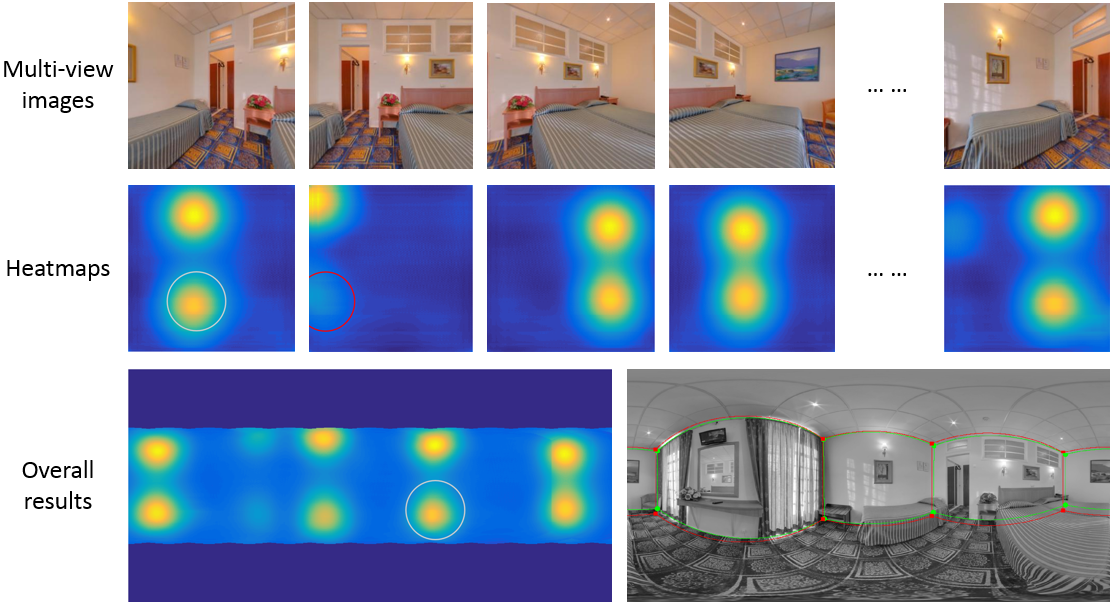
\includegraphics[width=\linewidth]{figs/results2.png}
	\caption{Our qualitative results on real data. We sum over the third dimension of the probability array $T$ for visulization. In the final result, the ground truth is shown in green and our prediction is shown in red. }
	\label{fig:results2}
\end{figure}

\begin{figure}
	\centering
	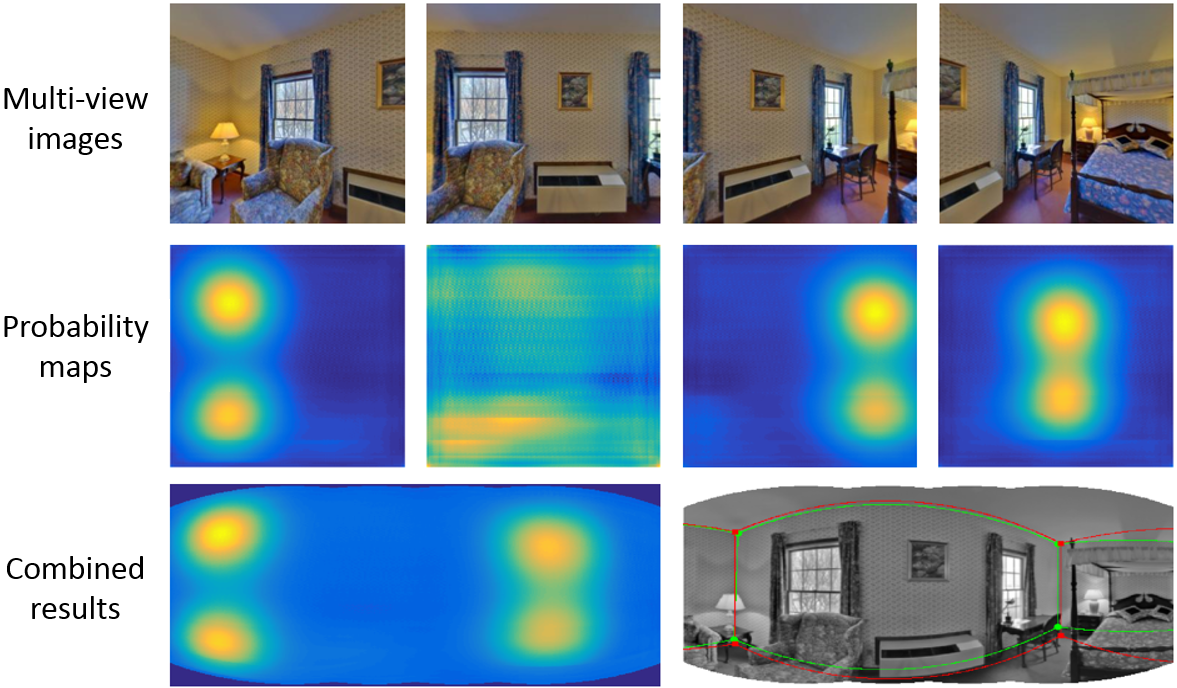
\includegraphics[width=\linewidth]{figs/partial2.png}
	\caption{A combined layout generated from four images. The predicted room corners are depicted by red points in the final result.}
	\label{fig:partial2}
\end{figure}


We also conduct experiments on the PanoContext dataset for quantitive comparison with previous panorama based methods, the same train/test split is adopted. 
%
Three standard metrics are adopted for evaluation: 3D Intersection over Union, Corner error and Pixel error. As shown in Tab. \ref{tab:PC}, our approach is comparable with panorama-based methods. 
%
We believe that the reason for the deficiency is that the FOV of each perspective image is much smaller than that of the panorama. Limited FOV may lead to the wrong focus, which then pollutes the overall prediction. 
%
To explore the effect of using different size of FOV, we use two settings during training and testing. For Multi-view-\ang{60}, we project the panorama into 24 perspective images with $FOV=\ang{60}$, while 8 directions around the vertical axis and 3 directions around the horizontal axis. For Multi-view-\ang{90}, we project the panorama into 12 perspective images with $FOV=\ang{90}$, all of them are horizontal and centered around the vertical axis. 
%
The quantitative results in Tab. \ref{tab:PC} demonstrate that larger FOV contribute to higher accuracy in overall prediction, which is consistent with our intuition. In fact, the panorama can be viewed as a special case that the FOV reaches its maximum.


%Experiments, three parts: one for different field of view (FOV), one for comparison with panorama based method, the last one for qualitative results.


%\begin{table}
%	\caption{Results of different FOV.}
%	\label{tab:FOV}
%	\begin{tabular}{cccc}
%		\toprule
%		FOV &3D IoU (\%)&Corner error (\%)&Pixel error (\%)\\
%		\midrule
%		 \ang{60} & XX & XX & XX\\
%	     \ang{90} & XX & XX & XX\\	
%		\bottomrule
%	\end{tabular}
%\end{table}


\begin{table}
	\caption{Quantitative results on PanoContext dataset.}
	\label{tab:PC}
	\begin{tabular}{cccc}
		\toprule
		Method&3D IoU (\%)& $\epsilon_{corner}$ (\%) & $\epsilon_{pixel}$ (\%)\\
		\midrule
		PanoContext \cite{zhang2014panocontext} & 67.23 & 1.60 & 4.55\\
		LayoutNet \cite{zou2018layoutnet} & 74.48 & 1.06 & 3.34\\
		Multi-view-\ang{60} & 53.39 & 3.35 & 10.15\\	
		Multi-view-\ang{90} & 61.98 & 2.75 & 6.73\\	
		\bottomrule
	\end{tabular}
\end{table}

\section{Conclusions}
In this paper, we propose a method to estimate the combined room layout based on multiple views. We design a concise representation for the room layout in the perspective image to simplify the learning process. Then we integrate the predicted room layout from different perpectives into a combined prediction using view transformations and a fusion strategy. The multi-view images can supplement each other and generate more accurate predicitons. We also achieve performance close to the panorama based methods on a panorama dataset. It is an encouraging attempt to estimate the room layout with larger FOV using multi-view images.

\comments{
\begin{acks}
	The authors would like to thank ...
\end{acks}
}

\comments{
\begin{figure}
	\centering
	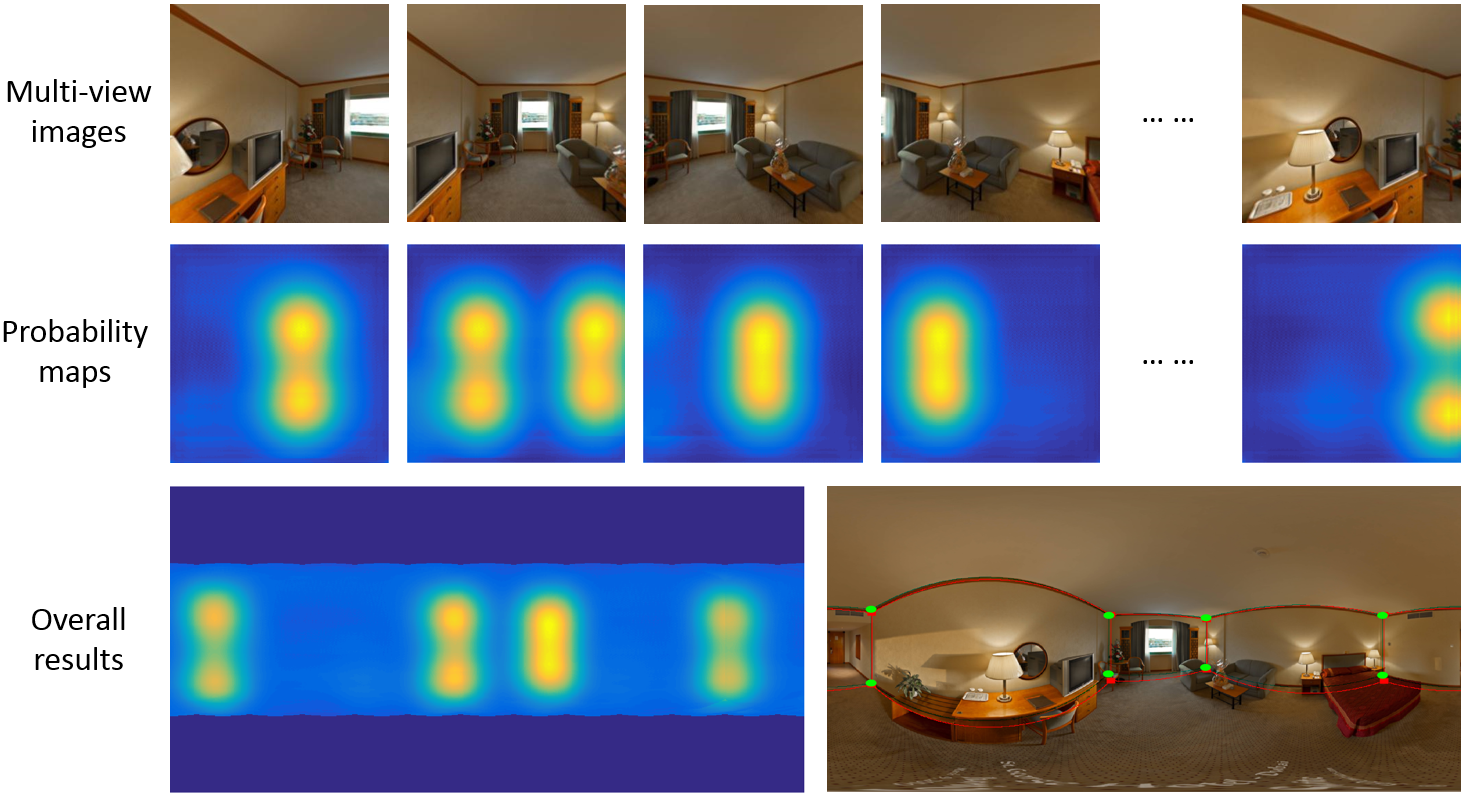
\includegraphics[width=\linewidth]{figs/results3.png}
	\caption{alternative/more results. }
	\label{fig:results3}
\end{figure}

\begin{figure}
	\centering
	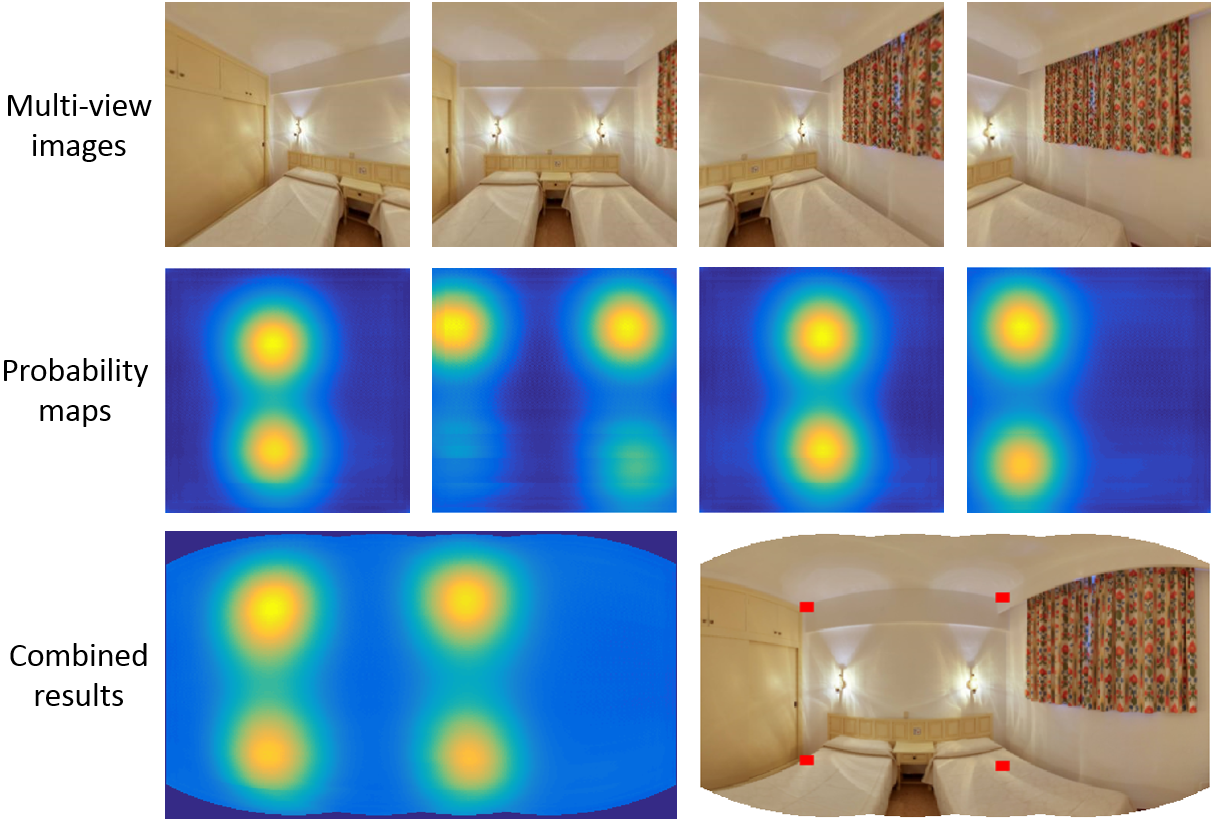
\includegraphics[width=\linewidth]{figs/partial1.png}
	\caption{alternative/more results for combined partial views. }
	\label{fig:partial1}
\end{figure}
}